%
% This is a borrowed LaTeX template file for lecture notes for CS267,
% Applications of Parallel Computing, UCBerkeley EECS Department.
% Now being used for CMU's 10725 Fall 2012 Optimization course
% taught by Geoff Gordon and Ryan Tibshirani.  When preparing 
% LaTeX notes for this class, please use this template.
%
% To familiarize yourself with this template, the body contains
% some examples of its use.  Look them over.  Then you can
% run LaTeX on this file.  After you have LaTeXed this file then
% you can look over the result either by printing it out with
% dvips or using xdvi. "pdflatex template.tex" should also work.
%

\documentclass[twoside]{article}
\setlength{\oddsidemargin}{0.25 in}
\setlength{\evensidemargin}{-0.25 in}
\setlength{\topmargin}{-0.6 in}
\setlength{\textwidth}{6.5 in}
\setlength{\textheight}{8.5 in}
\setlength{\headsep}{0.75 in}
\setlength{\parindent}{0 in}
\setlength{\parskip}{0.1 in}

%
% ADD PACKAGES here:
%

\usepackage{amsmath,amsfonts,graphicx}

%
% The following commands set up the lecnum (lecture number)
% counter and make various numbering schemes work relative
% to the lecture number.
%
\newcounter{lecnum}
\renewcommand{\thepage}{\thelecnum-\arabic{page}}
\renewcommand{\thesection}{\thelecnum.\arabic{section}}
\renewcommand{\theequation}{\thelecnum.\arabic{equation}}
\renewcommand{\thefigure}{\thelecnum.\arabic{figure}}
\renewcommand{\thetable}{\thelecnum.\arabic{table}}

%
% The following macro is used to generate the header.
%
\newcommand{\lecture}[4]{
   \pagestyle{myheadings}
   \thispagestyle{plain}
   \newpage
   \setcounter{lecnum}{#1}
   \setcounter{page}{1}
   \noindent
   \begin{center}
   \framebox{
      \vbox{\vspace{2mm}
    \hbox to 6.28in { {\bf EE302 - Feedback Systems
	\hfill Spring 2019} }
       \vspace{4mm}
       \hbox to 6.28in { {\Large \hfill Lecture #1 \hfill} }
       \vspace{2mm}
       \hbox to 6.28in { {\it Lecturer: #2 \hfill } }
      \vspace{2mm}}
   }
   \end{center}
   \markboth{Lecture #1}{Lecture #1}

   \vspace*{4mm}
}
%
% Convention for citations is authors' initials followed by the year.
% For example, to cite a paper by Leighton and Maggs you would type
% \cite{LM89}, and to cite a paper by Strassen you would type \cite{S69}.
% (To avoid bibliography problems, for now we redefine the \cite command.)
% Also commands that create a suitable format for the reference list.
\renewcommand{\cite}[1]{[#1]}
\def\beginrefs{\begin{list}%
        {[\arabic{equation}]}{\usecounter{equation}
         \setlength{\leftmargin}{2.0truecm}\setlength{\labelsep}{0.4truecm}%
         \setlength{\labelwidth}{1.6truecm}}}
\def\endrefs{\end{list}}
\def\bibentry#1{\item[\hbox{[#1]}]}

%Use this command for a figure; it puts a figure in wherever you want it.
%usage: \fig{NUMBER}{SPACE-IN-INCHES}{CAPTION}
\newcommand{\fig}[3]{
			\vspace{#2}
			\begin{center}
			Figure \thelecnum.#1:~#3
			\end{center}
	}
% Use these for theorems, lemmas, proofs, etc.
\newtheorem{theorem}{Theorem}[lecnum]
\newtheorem{lemma}[theorem]{Lemma}
\newtheorem{proposition}[theorem]{Proposition}
\newtheorem{claim}[theorem]{Claim}
\newtheorem{corollary}[theorem]{Corollary}
\newtheorem{definition}[theorem]{Definition}
\newenvironment{proof}{{\bf Proof:}}{\hfill\rule{2mm}{2mm}}

% **** IF YOU WANT TO DEFINE ADDITIONAL MACROS FOR YOURSELF, PUT THEM HERE:

\begin{document}

% Lecture Details
\lecture{7}{Asst. Prof. M. Mert Ankarali}

\par 

\section{Time Domain Analysis}

    \begin{minipage}[h]{0.5\linewidth}
    \begin{center}
      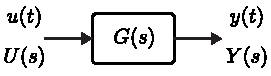
\includegraphics[width=0.9\textwidth]{sys}
    \end{center}
  \end{minipage}
    \begin{minipage}[h]{0.5\linewidth}
    \begin{center}
      \begin{align*}
      	Y(s) &= G(s) U(s)
	\\
	y(t) &= \mathcal{L} \lbrace G(s) U(s) \rbrace^{-1}
      \end{align*}
    \end{center}
  \end{minipage}
  
  Objective: 
  
\begin{itemize}
	\item Calculate $y(t)$ for different $u(t)$,
	\item Understand the relation between the parameters and output behavior.
\end{itemize}
    
    \subsection{First Order Systems}
    
    Simplest first order system is an integrator, which is also the fundamental block for higher order systems. 
    
    \begin{center}    
        \begin{minipage}[h]{0.5\linewidth}
    \begin{center}
      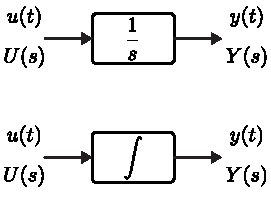
\includegraphics[width=0.9\textwidth]{int}
    \end{center}
  \end{minipage}
      \end{center}
      
      \textbf{Ex 1:} Compute the step-response of the integrator system, $G(s) = \frac{1}{s}$.
      
      \textbf{Solution:} We assume that initial conditions are zero
      
          \begin{minipage}[h]{0.7\linewidth}
    \begin{center}
      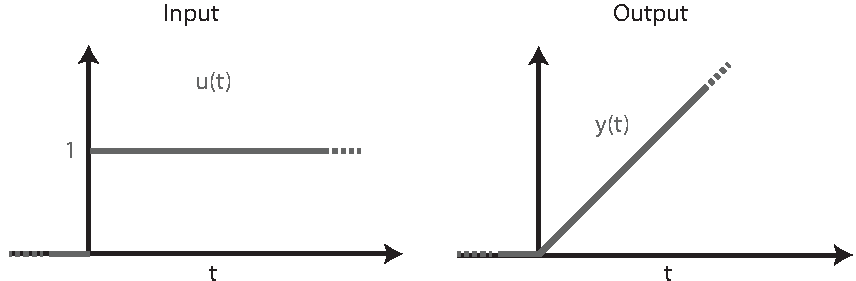
\includegraphics[width=1\textwidth]{signals}
    \end{center}
  \end{minipage}
    \begin{minipage}[h]{0.3\linewidth}
    \begin{center}
      \begin{align*}
      	U(s) &= \frac{1}{s} 
	\\
	Y(s) &= G(s) U(s) = \frac{1}{s^2}  
	\\
	y(t) &= \mathcal{L}^{-1}{ \frac{1}{s^2}  }
	\\
	&= t \ , \ \mathrm{for} \ t \geq 0
      \end{align*}
    \end{center}
  \end{minipage}
     
     \vspace{12pt}
     
     \textbf{Ex 2:} Compute the step-response of the following first order system
     
         \begin{minipage}[h]{0.7\linewidth}
    \begin{center}
      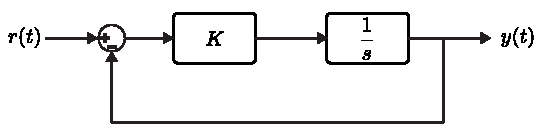
\includegraphics[width=1\textwidth]{firstex}
    \end{center}
  \end{minipage}
    \begin{minipage}[h]{0.3\linewidth}
    \begin{center}
      \begin{align*}
	G(s) &= \frac{K}{s+K} \
	\\
	Y(s) &= \frac{K}{s (s+K)} = \frac{K}{s (s+K)}
	\\
	&= \frac{A}{s} + \frac{B}{s+K}
      \end{align*}
    \end{center}
  \end{minipage}
  
  We can compute $A$ and $B$ as
  %
  \begin{align*}
  	A &= \lim_{s \to 0} \left[  s Y(s) \right] = \frac{K}{K} = 1
	\\
	B &= \lim_{s \to -K} \left[  (s+K) Y(s) \right] = \frac{K}{-K} = -1
   \end{align*}
%
Then, we can compute $y(t)$ as
%
  \begin{align*}
y(t) &= \mathcal{L}^{-1} \left\lbrace \frac{1}{s} - \frac{1}{s+K} \right\rbrace  
\\
&= \left[ 1 - e^{-K t} \right] \ , \ \mathrm{for} t \geq 0
\end{align*}

         \begin{minipage}[h]{0.5\linewidth}
    \begin{center}
      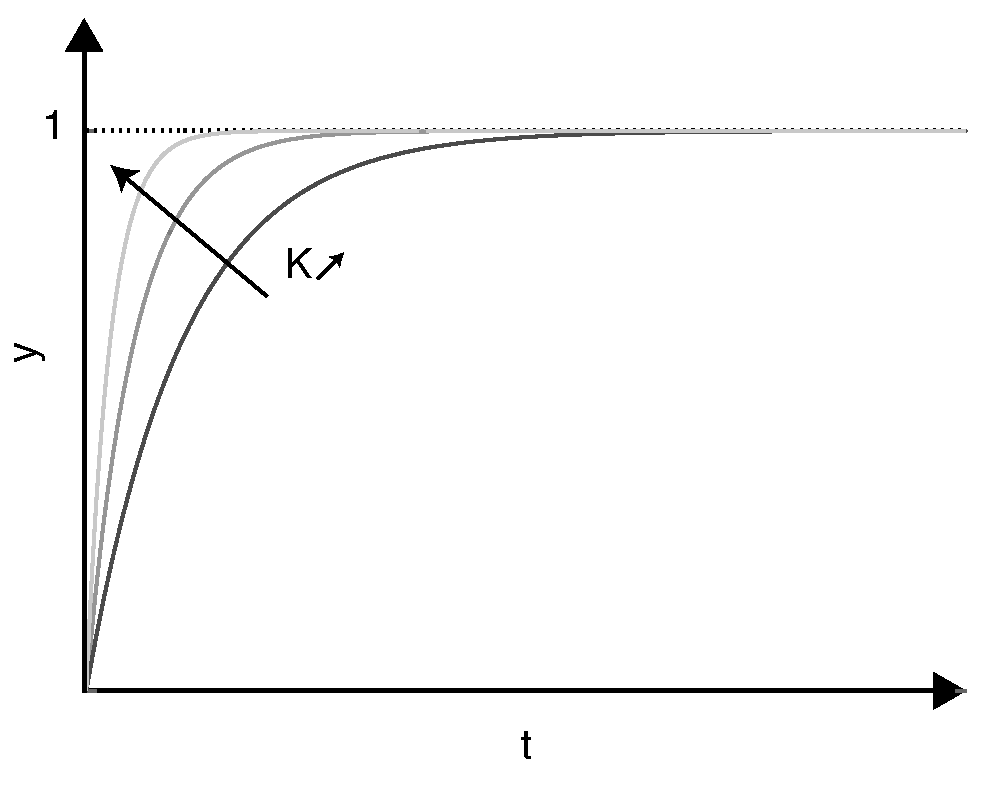
\includegraphics[width=1\textwidth]{step}
    \end{center}
  \end{minipage}
    \begin{minipage}[h]{0.5\linewidth}
        \begin{center}
          Proportional Controller
          %
      \begin{align*}
	\lim_{t \to \infty} y(t) &= 1
	\\
	\lim_{t \to \infty} e(t) &= \lim_{t \to \infty} (y(t) - u(t)) = 0
      \end{align*}
      Zero steady-state error $\forall K > 0$
      
      ``Convergence speed'' $ \nearrow$ as $K \nearrow$
          \end{center}
  \end{minipage}

\textbf{Ex 2:} Find the unit-ramp response for the same system
%
\begin{align*}
	Y(s) &= \frac{K}{s^2 (s+K)} 
	\\
	&= \frac{A}{s} + \frac{B}{s^2} + \frac{C}{s+K}
\end{align*}
%
$A$, $B$, and $C$ can be computed as
%
\begin{align*}
	C &= \lim_{s \to -K} \left[  (s+K) Y(s) \right] = \frac{1}{K} 
	\\ 
	B &= \lim_{s \to 0} \left[  s^2 Y(s) \right] = 1
	\\
	A &= \lim_{s \to 0} \frac{d}{d s} \left[  s^2 Y(s) \right] =
	 \lim_{s \to 0} \frac{d}{d s} \left[  \frac{K}{(s+K)}  \right] 
	=  \lim_{s \to 0} \left[  \frac{-K}{(s+K)^2}  \right] 
	= \frac{-1}{K}
\end{align*}
%
Then, we can compute $y(t)$ as
%
  \begin{align*}
y(t) &= \frac{-1}{K} + t + \frac{1}{K} e^{-K t} \ ,  \ \mathrm{for} \ t \geq 0
\\
y(t) &= t + \frac{-1}{K} \left[ 1 -  \frac{1}{K} e^{-K t} \right] \ ,  \ \mathrm{for} \ t \geq 0
\end{align*}
%
Note that $r(t) = t \ , \ \mathrm{for} \ t \geq 0$.

\vspace{12pt}

         \begin{minipage}[h]{0.5\linewidth}
    \begin{center}
      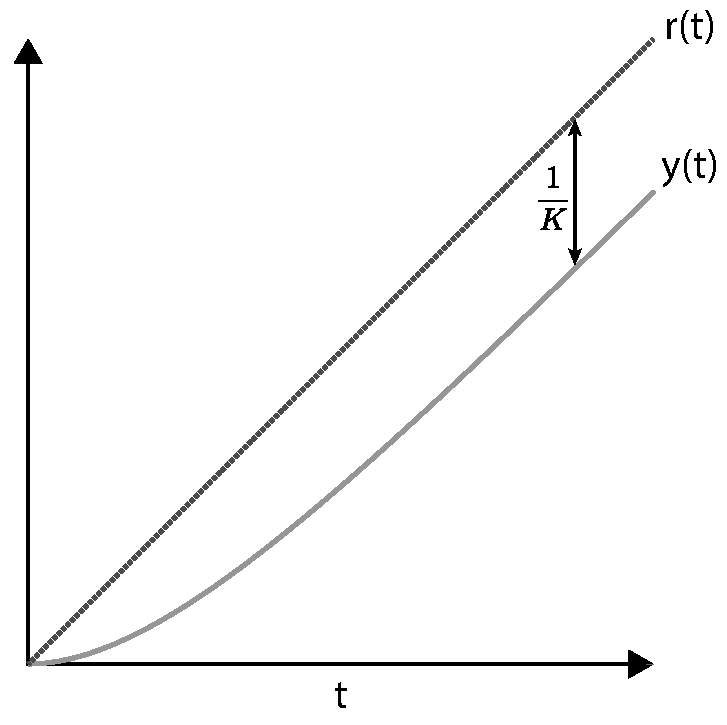
\includegraphics[width=1\textwidth]{ramp}
    \end{center}
  \end{minipage}
    \begin{minipage}[h]{0.5\linewidth}
        \begin{center}
          Proportional Controller
          %
      \begin{align*}
	&e(t) = r(t) - y(t) = \frac{1}{K} \left[ 1 -  \frac{1}{K} e^{-K t} \right]
	\\
	&\lim_{t \to \infty} e(t) = \frac{1}{K}
      \end{align*}
      Non-zero steady-state error 
      
      Steady-state error $ \searrow$ as $K \nearrow$
          \end{center}
  \end{minipage}
      
    
% **** This ENDS THE EXAMPLES. DON'T DELETE THE FOLLOWING LINE:
\end{document}